In this section, we describe the two experiments designed demonstrate how the ESI can be used to:
\begin{itemize} 
\item Quantify and visualize changes in the environment, and to what degree it accurately reflects these changes.
\item Estimate and predict AMCL's performance in rapidly changing environments.
\item Reduce AMCL's pose estimation error in rapidly changing environments by dynamically tuning its parameters.
\end{itemize}

\subsection{Real-world experiment} 
To demonstrate that the ESI works on a real robot in a real enviroment, and that it can be used to visualize changes in it, we used a MiR100 AMR as the platform.
The venue is the production hall of a packaging and labeling company. It is chosen because it represents the type of environment where AMCL often struggles;
it is constantly developing, and most of the time, the the majority of what the robot is able to see consists of transient objects, as seen in Figure X.
\subsubsection{Setup} A small section of the hall is mapped, using the native mapping functionality (based on ROS1 cartographer). We placed two waypoints, Start and Finish.
The task of the robot is simply to move from Start to Finish. In order avoid disrupting their production, instead of moving the items around, we first recorded the map,
and then gradually edit the map manually. This will create the same map-environment disagreements. The robot will be tested in four scenarios: 1) No, 2) light, 3) moderate 
and 4) severe changes. Each scenario will be executed 5 times, and the ESI recorded for all runs. When the robot reaches the end, its pose error is obtained from a reference
coordinate system on the floor. 
\subsubsection{Results}


\begin{table}[!h]
    \begin{center}
    \caption{\footnotesize{ESI results for the real-world experiment. 1) No changes, 2) Light changes, 3) Moderate changes, 4) Significant changes. Units for rows with a * is \textnormal{[mm]} and \textnormal{[°]}.}}
    \adjustbox{width=\textwidth/2,center}{%
    \begin{tabular}{|c|c|c|c|c|c|c|c|c|c|}
    \hline
    \textbf{Scenario} & \multicolumn{2}{c|}{\textbf{1})} & \multicolumn{2}{c|}{\textbf{2)}} & \multicolumn{2}{c|}{\textbf{3)}} & \multicolumn{2}{c|}{\textbf{4)}} \\
    \hline
    \textbf{* Pose RMSE} & 22.4 & 2.4 & 17.5 & 2.1 & 21.1 & 2.4 & N/A & N/A \\
    \hline
    \textbf{* Pose Std. dev.} & 25.1 & 2.7 & 19.5 & 1.1 & 20.5 & 1.0 & N/A & N/A \\
    \hline
    \textbf{ESI mean} & \multicolumn{2}{c|}{0.94} & \multicolumn{2}{c|}{0.64} & \multicolumn{2}{c|}{0.46} & \multicolumn{2}{c|}{0.22} \\
    \hline
    \textbf{ESI std. dev.} & \multicolumn{2}{c|}{0.04} & \multicolumn{2}{c|}{0.12} & \multicolumn{2}{c|}{0.10} & \multicolumn{2}{c|}{0.09} \\
    \hline
    \end{tabular}%
    }
    \label{table:real_world_esi_results}
    \end{center}
    \end{table}

\begin{figure}[H]
    \centerline{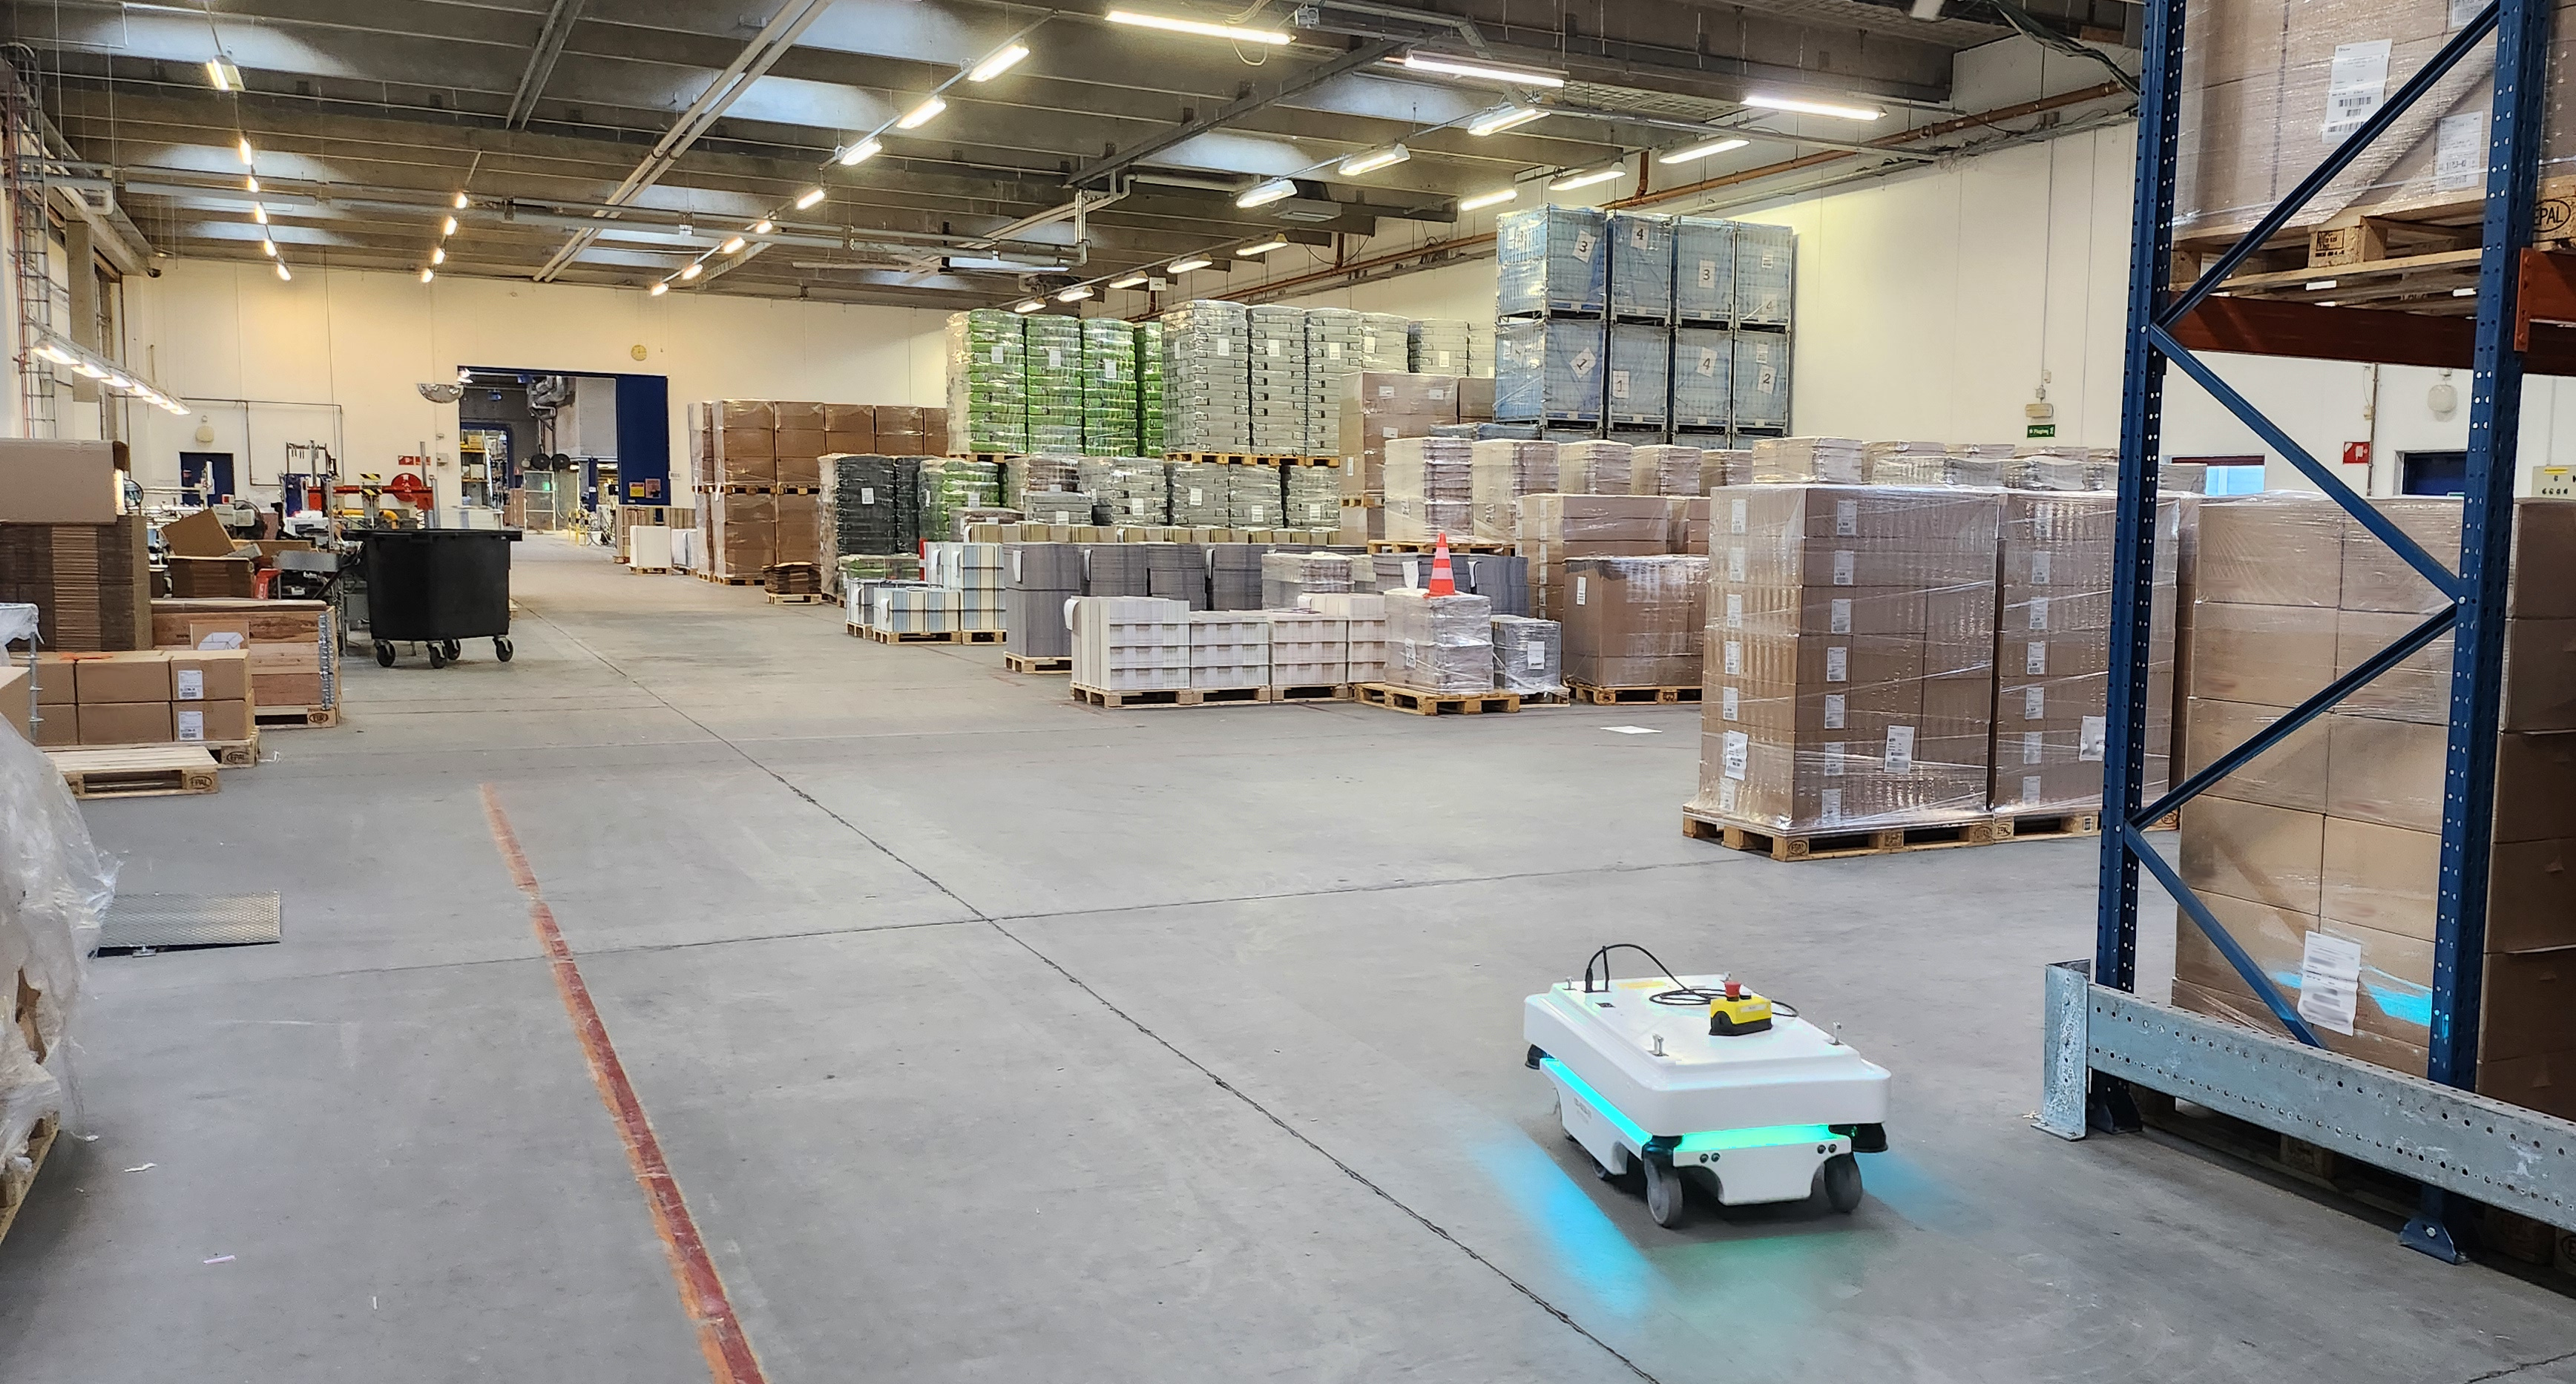
\includegraphics[width=\columnwidth]{figures/schur_img_1.png}}
    \caption{Example of a figure caption.}
    \label{fig2}
\end{figure}



\subsection{Simulation experiment}
...

